%!TeX root=../tese.tex
%("dica" para o editor de texto: este arquivo é parte de um documento maior)
% para saber mais: https://tex.stackexchange.com/q/78101

%% ------------------------------------------------------------------------- %%

% "\chapter" cria um capítulo com número e o coloca no sumário; "\chapter*"
% cria um capítulo sem número e não o coloca no sumário. A introdução não
% deve ser numerada, mas deve aparecer no sumário. Por conta disso, este
% modelo define o comando "\unnumberedchapter".
\unnumberedchapter{Introduction}
\label{cap:introducao}

\enlargethispage{.5\baselineskip}

As defined by \citet{matsakis2014rust} the Rust \index{Rust} programming language is a modern
systems programming language focused on safety, speed and concurrency. It compares
to C++ in terms of mapping directly to hardware, but it is safer to use thanks to
the guarantees it's static type system provides. The language has been successfully
used on a number of different domains, including astrophysics \citep{blanco2016can}
and operating system kernels development \citep{levy2017case}.

The Rust compiler is a complex piece of software, with many different components.
It is written in Rust itself, making it a self-hosted language, and it is composed
of a Rust front-end, a LLVM middle-end and a LLVM back-end.\index{LLVM}

As described by the \citet{rustc-dev-guide} the front-end is responsible for parsing
the source code, desugaring, checking and validating it, and generating a first intermediate
representation of the code, called High-level Intermediate Representation (HIR). \index{HIR}
After this, the middle-end is responsible for lowering the HIR to a lower-level representation
called Middle-level Intermediate Representation (MIR) \index{MIR} by doing type checking. On the next step,
the compiler enforces the borrow checking rules, which are one of the main features of the Rust language,
and executes some initial optimizations, finally lowering the MIR to an IR called LLVM IR. From here on,
the LLVM middle-end enters and starts to transform the LLVM IR into a more optimized version of itself.
Finally, the LLVM back-end is responsible for lowering the LLVM IR to the target machine assembly code. It's important
to notice that the Rust compiler is not tied to the LLVM compiler framework, but it is the most used back-end.
A high-level overview of the Rust compilation pipeline can be seen on Figure~\ref{fig:rustc-pipeline}.

\begin{figure}[ht]
    \centering
    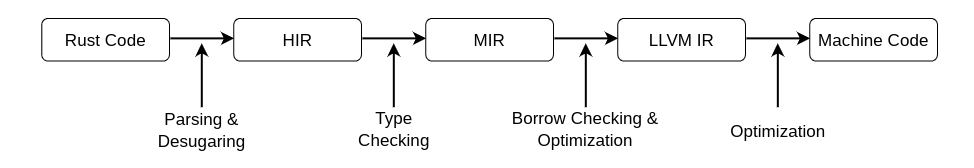
\includegraphics[width=1\textwidth]{figuras/rustc.png}
    \caption{Overview of the Rust compilation pipeline}
    \label{fig:rustc-pipeline}
\end{figure}


%% ------------------------------------------------------------------------- %%
\unnumberedsection{LLVM Optimizations}
\label{sec:consideracoes_preliminares}

As \citet{lattner2004llvm} describe, the LLVM \index{LLVM} compiler framework is a collection of modular and reusable compiler
and toolchain technologies. It is designed to be used as a back-end for a wide variety of programming languages,
and it is used as the middle-end and back-end for the Rust compiler. One of the central features of LLVM is it's intermediate
representation (IR), which is a low-level programming language similar to assembly. The IR is designed to represent
programs in a form that is independent of the source programming language, and it is used as the common language between
the different components of the compiler. The IR is also designed to be a target of both static and dynamic compilation
techniques, and it is suited for optimization and analysis.

The LLVM IR is a typed, static single assignment (SSA) \index{SSA} representation of a program, designed to be used in three
different forms: in memory, as an on-disk bitcode representation (suitable for fast loading by a Just-In-Time compiler),
and as a human readable assembly language representation. The LLVM IR is defined in three different levels of abstraction:
the high-level virtual instruction set, the low-level virtual instruction set, and the concrete representation. The high-level
virtual instruction set is the most abstract representation, and it is used by the front-end of the compiler. The low-level
virtual instruction set is a more concrete representation, and it is used by the middle-end of the compiler. The concrete
representation is the most concrete representation, and it is used by the back-end of the compiler. The LLVM IR is a
static single assignment representation, which means that each value is assigned only once, and it is defined before it is used.
This property simplifies the analysis and transformation of the code, and it is a requirement for some optimizations.

There is a set of passes that can be applied to the LLVM IR, and they are divided into two categories: analysis
passes and transformation passes. Analysis passes are used to obtain information about the code, without changing it.
That information can be queried by a transformation pass or by other analysis passes. The result of an analysis pass is always cached
and will only be invalidated if the unit of IR used by it has changed.
Transformation passes are used to change the code in some way. The operation is done in-place and always leaves the IR in a valid state.
A transformation pass can depend on the result of an analysis pass and will only run after querying it.

Table~\ref{tab:analysis} describe all LLVM IR analysis passes, and Table~\ref{tab:transformation} the transformation passes, that are available in the LLVM 16.0.6 release.

%% ------------------------------------------------------------------------- %%
\unnumberedsection{Adaptive Compilation}

As described by \citet{cooper2005acme} adaptive compilation is a technique that allows a compiler to increase the performance
of a program by monitoring it's execution and recompiling it with different optimizations. The compiler can use the information
gathered during the execution to decide which optimizations to apply, and it can also use the information to decide when to
recompile the program. The compiler can also use the information to decide when to stop recompiling the program, and it can
also decide to recompile the program with less optimizations if it detects that the program is not benefiting from them. As such,
an adaptive compiler can be seen as a compiler that is able to adapt to the behavior of the program through a compile-execute-analyze feedback loop,
based on some well defined performance metric, such as binary size or execution time. The main task of an adaptive compiler becomes then to find
the best set of optimizations for a given program.

The main advantage of adaptive compilation is that it allows the compiler to make decisions based on the actual behavior of the
program, instead of making decisions based on the static analysis of the code. This allows the compiler to make better decisions
and to generate better code. The main disadvantage of adaptive compilation is the large amount of time it takes to walk over the search space of
all optimization passes.



%% ------------------------------------------------------------------------- %%